\section{Results}

As input our system takes a source video and a single target image of a face. It generates a dynamic texture of the target image for a 3D model and retargets the source mesh onto the single input image, inferring details such as wrinkles and the inner mouth region.  Our results can be seen in Fig.~\ref{fig:result}. More results can be seen in the supplementary material.


\paragraph{Reenactment: Comparison To Previous Works}

When given only a single image as a target input, \cite{f2f} can only generate static textures and does not capture any of the wrinkles or inner mouth details that our system captures as seen in Fig.~\ref{fig:result}. 

An example of methods like \cite{f2f} that do not use our inference model, thereby producing less detailed results when there is only a single target image as input, can be seen in Fig.~\ref{fig:wrinkles}.


\begin{figure}[th]
	\centering
	\includegraphics[width=1.0\linewidth]{figures/wrinkles/example_crop.png}
	\caption{Wrinkle animations from a single neutral target input image. In each row, the pair of images on the left shows the facial animation achieved using a static texture generated by a multilinear fitting such as~\cite{f2f}. The pair of images on the right shows the facial animation achieved using the dynamic texture generated by our inference model. Note that the images on the right are capable of generating detailed wrinkles and filling the inner mouth cavity.}~\label{fig:wrinkles}
	\vspace{-0.2in}
\end{figure}

\paragraph{Quantitative Evaluation}

To further validate our approach, we performed quantitative evaluation against an alternative, more direct approach to dynamic texture synthesis. Given an image of the source subject making a facial expression and a and neutral frame of the same subject, we apply the difference between these two images to the neutral frame of the target subject. We performed this test for 20 expression sequences, each 900 frames long, in which each of 5 test subjects are retargeted to one another. The test sequences have been synchronized in the same manner as the training data, thereby providing ground truth expressions for each retargeted sequence. The results, shown in Table ~\ref{table:paris}, demonstrate that our method synthesizes textures that are closer to the ground truth texture data. Furthermore, we note that while this more naive approach to texture synthesis (which we call ``direct delta transfer'') is simpler to implement and can synthesize wrinkles and other details on the target subject, simply applying these differences to the target subject does not account for geometric dissimilarity in the faces of the subjects, and thus it typically generates results that are far more uncanny and implausible than our approach.

%% \paragraph{Composition: Comparison To Previous Works}

%% \cite{replace} is currently the state-of-the-art with respect to face composition, and their results are shown in Fig.~\ref{replaceres}. Our results for composition in Fig.~\ref{fig:result} are comparable to theirs, but we only need a single target image as input while they need a video sequence.

%% \begin{figure}[th]
%% \begin{center}
%%    \includegraphics[height=90px]{figures/results/daleaa.png}
%%    \includegraphics[height=88px]{figures/results/dalebb.png}
%% \end{center}
%%    \caption{\protect\cite{replace} takes two video inputs and can do face replacement as shown in this figure. Our results are comparable to the results in this figure, but we are only using a single target image as input. Furthermore, \protect\cite{replace} cannot handle only a single target image as input.}
%%    \vspace{-0.05in}
%% \label{replaceres}
%% \end{figure}

% TODO: reference to the table. Did we take average over all the images? The names of the
% methods in the table should be fleshed out. The caption should be fleshed out.
\begin{table}[h!]
\begin{center}
\resizebox{.45\textwidth}{!}{%
  \begin{tabular}{ l  c  c c}
    \hline
    Method & Mean L1 Loss & Mean L2 Loss & SSIM \\ \hline
    \emph{Our result} & 1360 &  152 & 0.8730 dB\\ \hline
    \emph{Direct delta transfer} & 1790  & 211 & 0.8150 dB\\ \hline
\end{tabular}}
\end{center}
\caption{Quantitative evalution against a more direct texture synthesis approach.}
\vspace{-0.2in}
\label{table:paris}
\end{table}


\setlength{\tabcolsep}{3pt}
\begin{figure*}[th]
	\centering
	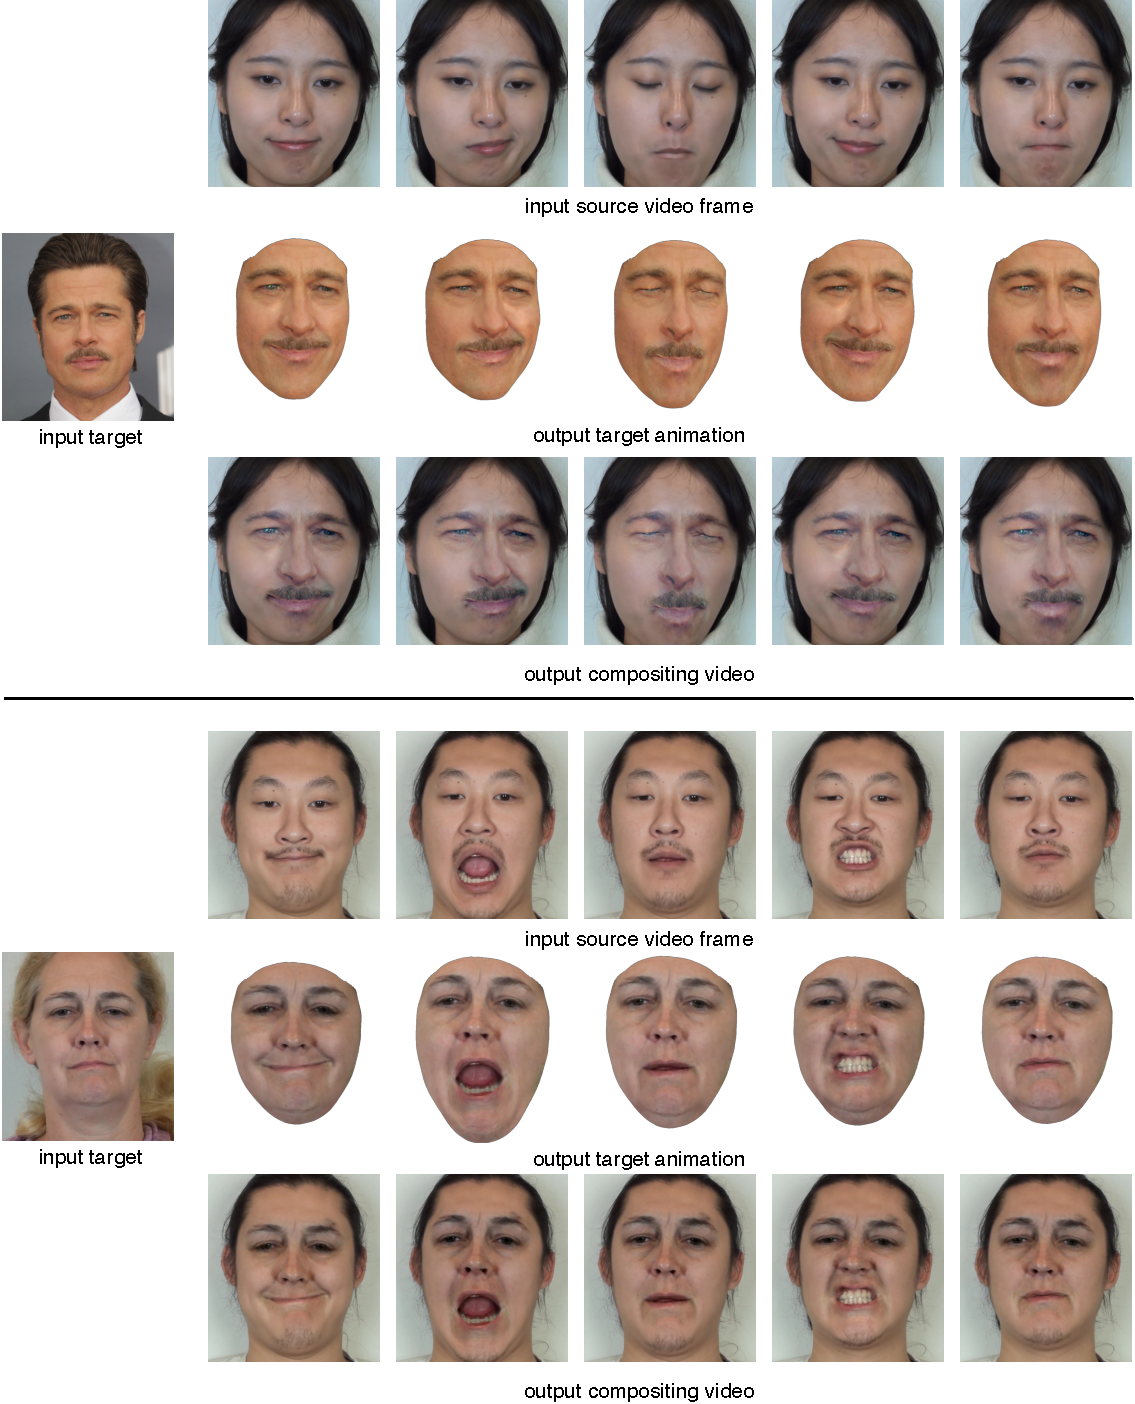
\includegraphics[width=.93\linewidth]{figures/results/figure6.pdf}
	\caption{Two sample results of our method. Top row of each example shows the source video sequence. Middle row shows the target single-frame input and the animated retargeted faces. Bottom row shows the compositing result.}
\end{figure*}

